\documentclass[peerreview]{IEEEtran}
\usepackage{cite} % Tidies up citation numbers.
\usepackage{url} % Provides better formatting of URLs.
\usepackage[utf8]{inputenc} % Allows Turkish characters.
\usepackage{booktabs} % Allows the use of \toprule, \midrule and \bottomrule in tables for horizontal lines
\usepackage{graphicx}
\usepackage{xcolor}

\usepackage{listings}

\usepackage{hyperref}

\definecolor{mygreen}{rgb}{0,0.6,0}
\definecolor{mygray}{rgb}{0.5,0.5,0.5}
\definecolor{mymauve}{rgb}{0.58,0,0.82}

\lstdefinestyle{CStyle}{
  belowcaptionskip=1\baselineskip,
  breaklines=true,
  frame=L,
  xleftmargin=\parindent,
  language=C,
  showstringspaces=false,
  basicstyle=\footnotesize\ttfamily,
  keywordstyle=\bfseries\color{green!40!black},
  commentstyle=\itshape\color{purple!40!black},
  identifierstyle=\color{blue},
  stringstyle=\color{orange},
}

\hyphenation{op-tical net-works semi-conduc-tor} % Corrects some bad hyphenation 

\begin{document}
%\begin{titlepage}
% paper title
% can use linebreaks \\ within to get better formatting as desired
\title{Laboratory of Innovative wireless platforms for the internet of things}

% author names and affiliations

\author{a.a. 2018 – 2019 \\
Daniele Castro S253244 \\
Group number: 8
}
\date{13/07/2019}

% make the title area
\maketitle
\tableofcontents
\listoffigures
%\end{titlepage}

\IEEEpeerreviewmaketitle
\begin{abstract}
The project is a simple to use script written in JavaScript that allows the user to know in advance whether to put a transmitting antenna in a specific place or not.
\end{abstract}
\section{Introduction}
The marker represents the transmitting antenna and the \textcolor{red}{red} and \textcolor{black}{black} spots represents possible retrieving antenna positions. If a spot is red, it means that in that place a retrieving antenna can retrieve the electromagnetic radiation from the transmitting antenna, not vice versa.
\begin{figure}[!ht]
\centering
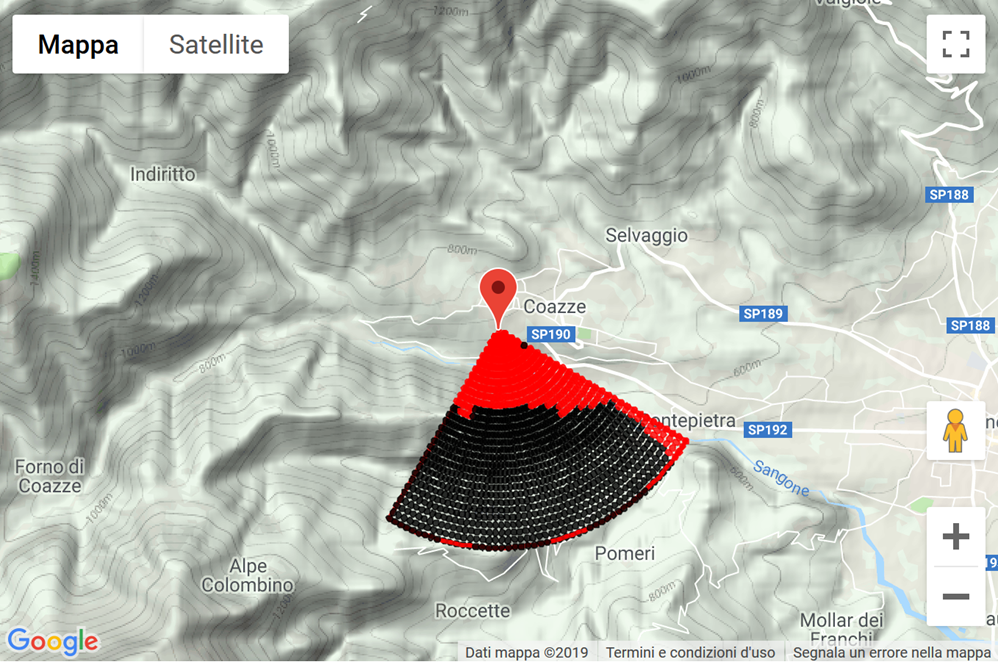
\includegraphics[width=1.0\columnwidth]{project_finished} 
\caption{obtained final result}
\label{fig_project_finished}
\end{figure} 
\section{Background}
Many parameters can be modified in order to give the best user experience in the \textbf{initMap()} function.
Configuration parameters:
\begin{itemize}
\item \textbf{radius} is the radius of the cone
\item \textbf{startAngle} and endAngle regulates the opening of the cone
\item \textbf{antennaHeight} is the height of the transmitting antenna
\item \textbf{retrieverHeight} is the height of the retrieving antenna
\item \textbf{samples} is the number of spots per path
\item \textbf{angleStep} is the angle between two paths
\end{itemize}
\pagebreak
Here can be better seen how \textbf{startAngle} and endAngle works:
\begin{figure}[!ht]
\centering
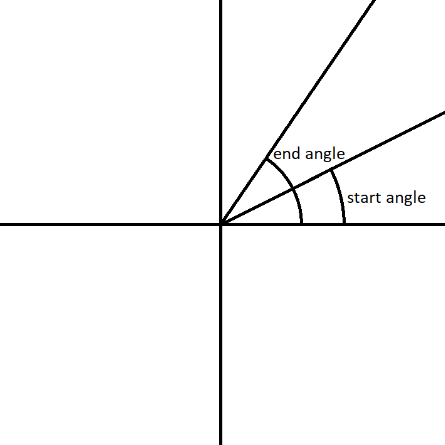
\includegraphics[width=0.8\columnwidth]{startangle} 
\caption{start angle and end angle behaviuor}
\label{fig_startangle}
\end{figure}
\\\textbf{retrieverHeight} is the height of the retrieving antenna and is summed to the height of each spot in the map because it is supposed that the user wants to see if placing a retrieving antenna in whatever place with a given height will work or the electromagnetic radiation will not achieve the retrieving antenna.
To better understand the meaning of \textbf{samples} and \textbf{angleStep} This picture can be useful:
\begin{figure}[!ht]
\centering
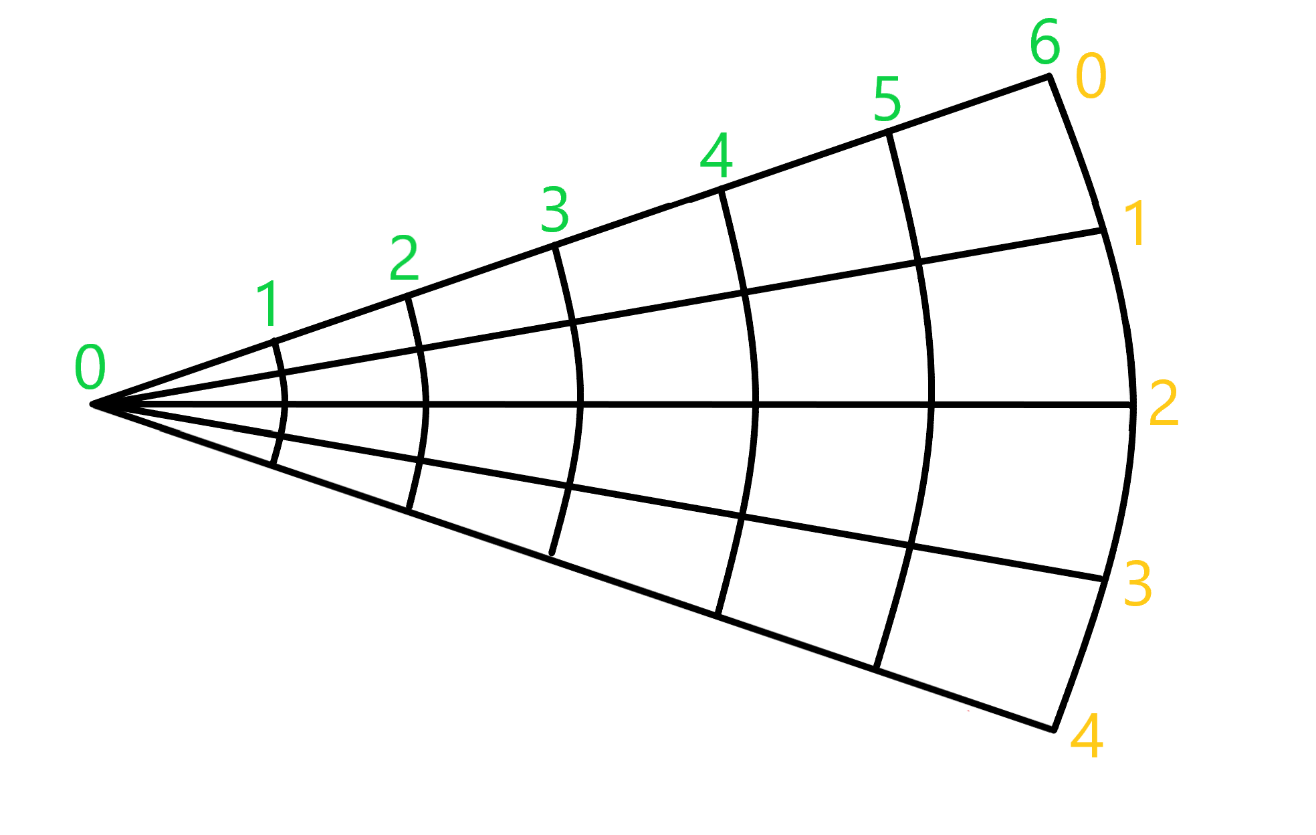
\includegraphics[width=0.85\columnwidth]{coneWithNumbers} 
\caption{map cone numbered}
\label{fig_coneWithNumbers}
\end{figure}
\\\textcolor{orange}{Orange} number represents paths and \textcolor{green}{green} numbers represents each single spot in a path; exception made for spot 0 that is the centre (the transmitting antenna position). Between two orange paths there is the \textbf{angleStep}.
\textbf{samples} is the number of green spots.
\section{Brief HGT file format explanation}
A file with the HGT file extension is a Shuttle Radar Topography Mission (SRTM) Data file. It contains digital elevation models, which are 3D pictures of a surface (usually a planet).
\begin{figure}[!ht]
\centering
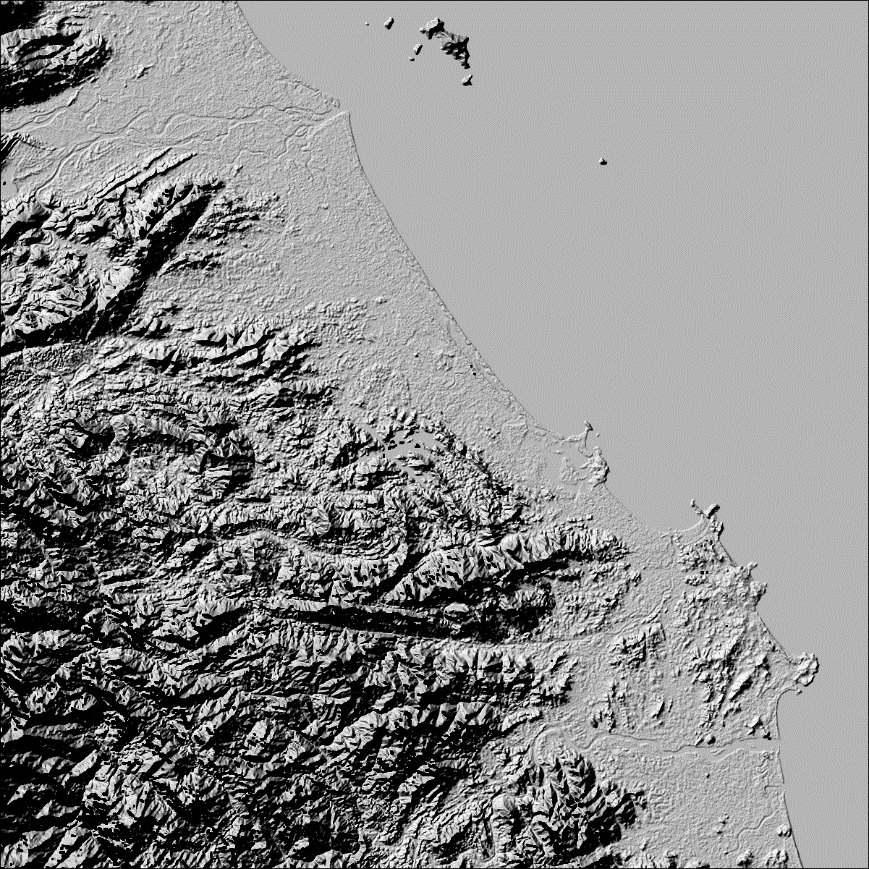
\includegraphics[width=1\columnwidth]{hgtPicture} 
\caption{HGT file converted into a picture}
\label{fig_hgtPicture}
\end{figure}
\\They are obtained during the Shuttle Radar Topography Mission (SRTM) by NASA and the National Geospatial-Intelligence Agency (NGA). "HGT" is just an abbreviation for "height". HGT file is normally named with the longitude and latitude that the image pertains to, within one degree. For example, the file N33W177.hgt would indicate that it includes data for latitudes 33 to 34 North and longitudes 177 to 178 West. SRTM data are distributed in two levels: SRTM1 (for the U.S. and its territories and possessions) with data sampled at one arc-second intervals in latitude and longitude, and SRTM3 (for the world) sampled at three arc-seconds (our case). Data are divided into one by one-degree latitude and longitude tiles in "geographic" projection, which is to say a raster presentation with equal intervals of latitude and longitude in no projection at all but easy to manipulate and mosaic. Height files are signed two-byte integers. The bytes are in Motorola "big-endian" order with the most significant byte first. Heights are in meters referenced to the WGS84/EGM96 geoid. Data voids are assigned the value of -32768. SRTM1 files are $3601*3601*2$ bytes long and SRTM3 files are $1201*1201*2$ bytes long.
\section{Custom API}
Since Google blocks its own services when too many requests are made within a second, A custom API had to be developed in order to make this project usable with a discrete number of samples.
These custom APIs are made of five functions:
\begin{itemize}
\item \textbf{do\_interpolation()}
\item \textbf{init\_interpolation()}
\item \textbf{reverse()}
\item \textbf{pointsAlongPath()}
\item \textbf{getElevationAndPoints()}
\end{itemize}
They work like this:\\
\textbf{init\_interpolation()} reads a given SRTM3 HGT file and generates a matrix containing all the height samples in the HGT file. Every time an height sample is extracted from the file \textbf{reverse()} function is called to swap the two bytes that makes the sample: it converts big-endian samples in little-endian ones. After this initialization process a \textbf{matrixObjct} is made and passed to the others API functions. This object contains the matrix extracted from the HGT file and the number of rows and columns.
\textbf{do\_interpolation()} is the function that does the interpolation. To make the interpolation possible \textbf{init\_interpolation()} filled the matrix like in the following picture:
\begin{figure}[!ht]
\centering
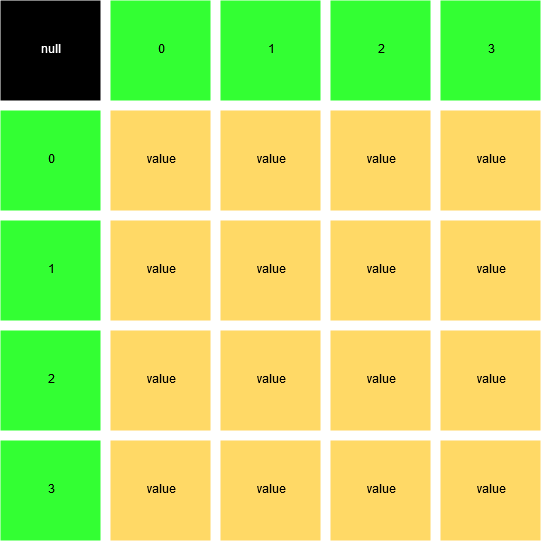
\includegraphics[width=1\columnwidth]{interpolationMatrix} 
\caption{interpolation matrix}
\label{fig_interpolationMatrix}
\end{figure}
\\\textbf{do\_interpolation()} also redirects to the proper file matrix the request of a given point coordinates.
\textbf{pointsAlongPath()} it is a simple function that gives a certain number of equidistant samples within a path.
Finally \textbf{getElevationAndPoints()} is the function that emulates the behaviour of the Google’s \textbf{getElevationAndPoints()} it calls \textbf{pointsAlongPath()} and returns an array of objects that contains the height and the coordinates of each point.
\section{Proposed Solution}
Script functions are:
\begin{itemize}
\item \textbf{initMap()}
\item \textbf{displayPathElevation()}
\item \textbf{makeCircle()}
\item \textbf{plotElevation()}
\item \textbf{plotElevation2()}
\item \textbf{getHeight()}
\item \textbf{onStraightSight()}
\end{itemize}
In the \textbf{initMap()} function few parameters can be tuned, like explained at the beginning, and the initialization function \textbf{displayPathElevation()} is called. Here \textbf{makeCircle()} creates a certain number of paths and calls \textbf{plotElevation()} that begins the recursion.\\
The code is synchronously run and made recursive because, in this way, it can be easily upgraded in an asynchronous algorithm. Asynchronous algorithms are optimal for web services since they allow multiple part of the algorithm to be run separately in parallel in different threads.
The recursion is made by \textbf{plotElevation()} and \textbf{plotElevation2()} To better explain how they work the following picture can be seen:
\begin{figure}[!ht]
\centering
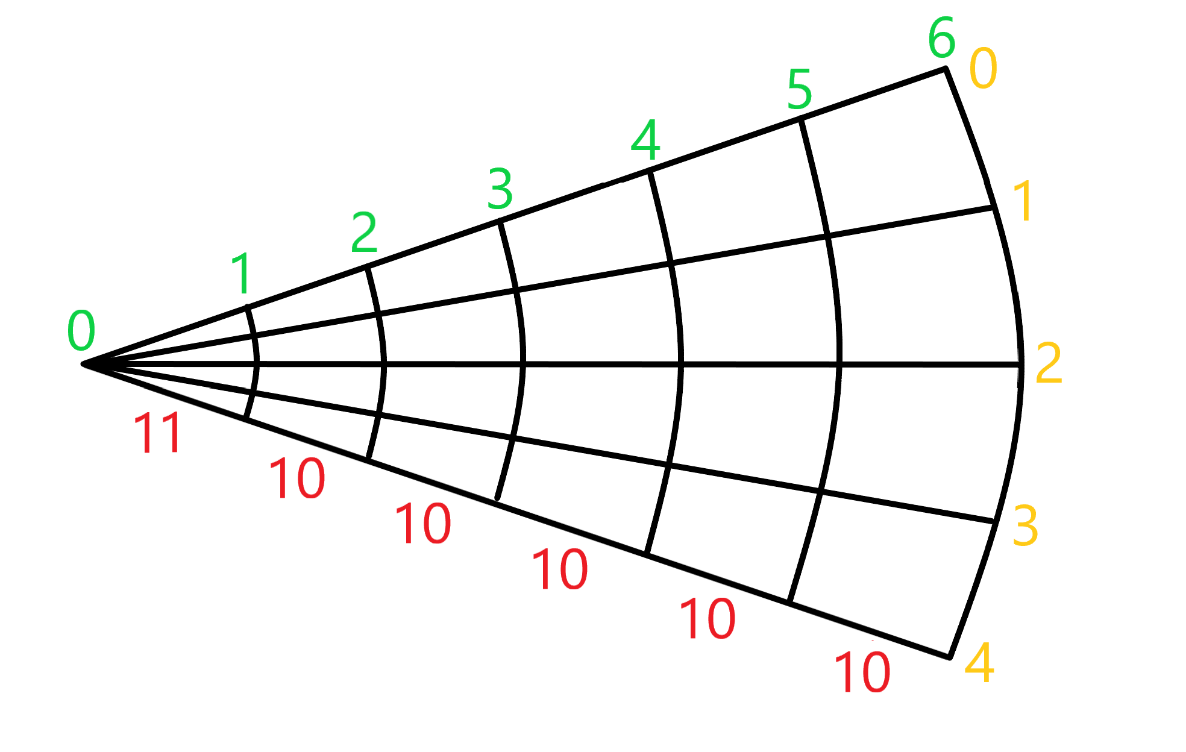
\includegraphics[width=1\columnwidth]{coneWithNumbers2} 
\caption{map cone numbered}
\label{fig_coneWithNumbers2}
\end{figure}
\\\textbf{plotElevation(}) increments the \textbf{cnt} recursion counter. \textbf{cnt} goes from 0 to the total number of \textcolor{orange}{orange} paths. So a \textbf{‘samples‘} number of \textcolor{green}{green} points are requested to be generated by \textbf{pointsAlongPath()}. For each of these points \textbf{plotElevation2()} is called and it increments the \textbf{i} recursion counter variable. It calls \textbf{getElevationAndPoints()} that is asked to generate $11+(10*(i-1))$ \textcolor{red}{red} number of samples along a path starting from the centre. All of these samples are passed through an array to \textbf{getHeight()} and  \textbf{onStraightSight()} that will, respectively, sum the earth curvature to the current heights array and calculate whether if a given point can be achieved by the electromagnetic radiation or not.
\pagebreak
\\Here follows a graphical explanation of what said:
\begin{figure}[!ht]
\centering
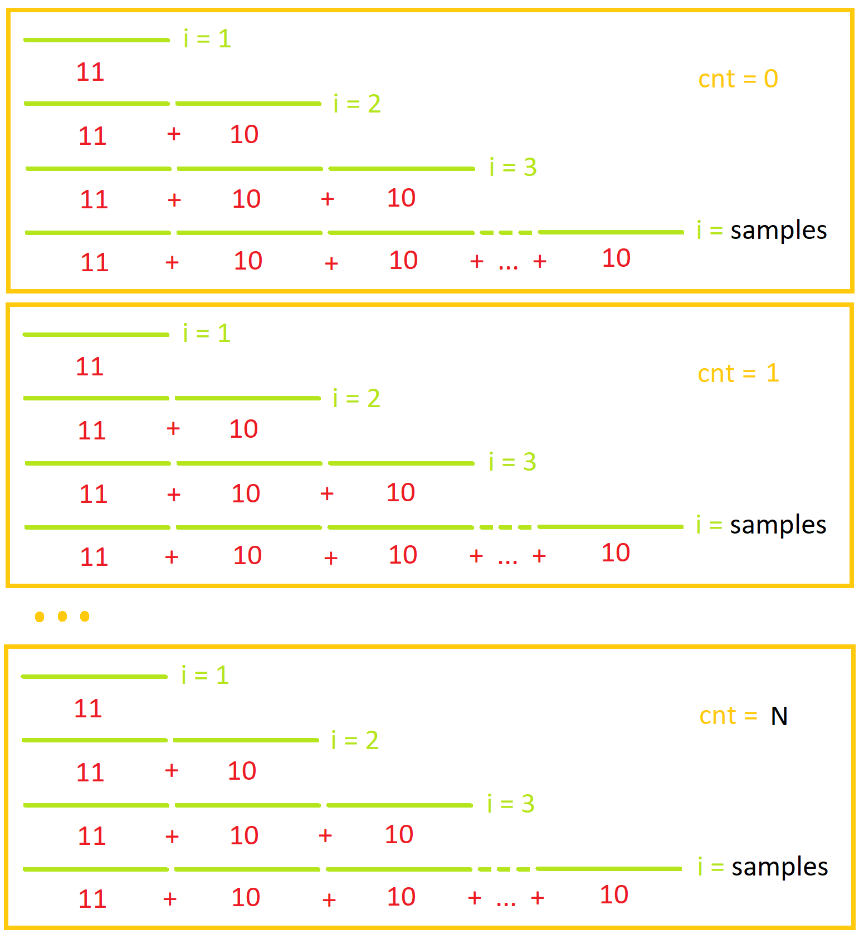
\includegraphics[width=1\columnwidth]{algorithm} 
\caption{graphical explanation of the algorithm}
\label{fig_algorithm}
\end{figure}\\
\section{Conclusions}
In this discussion I have accomplished the assignment requested. I would like to reuse this script even for further uses since it has been made flexible and scalable.

\begin{thebibliography}{1}
\bibitem{SRTM Documentation}
SRTM Documentation (best viewed with mono-spaced font, such as courier), [txt] Available at:\\ \href{https://dds.cr.usgs.gov/srtm/version1/Documentation/SRTM_Topo.txt}{\underline{\textcolor{blue}{Link}}}.\\Accessed on: July 13, 2019.
\bibitem{Google API}
Google maps API, Available at:\\ \href{https://cloud.google.com/maps-platform/}{\underline{\textcolor{blue}{Link}}}.\\Accessed on: July 13, 2019.
\bibitem{Interpolation script}
Interpolation javascript script, Available at:\\ \href{https://www.danbp.org/p/en/node/53}{\underline{\textcolor{blue}{Link}}}.\\Accessed on: July 13, 2019.
\end{thebibliography}

\end{document}